\section{Introduction}\label{introduction}

This report analyses the effectiveness of a using a PID controller
derived in Phase 2 on a Quanser-rig. Before testing the controller on a
Quanser-rig, nonlinearities were added to the simulation. Through using
a design process to improve the controller response, new control
objectives were met, then implemented on the Quanser-rig. The following
report discusses both the design process, testing results and any
observations made through creating an effective controller for the
Quanser-rig.

The following transfer function was used to design the controller, taken
from Phase 1:

\begin{align*}
&\text{$2^{nd}$ Order: }k \cdot \frac { 1.109\cdot \frac{180} {\pi} }{ s^2 + 0.1313s +1.109 }
&&\text{$1^{st}$ Order: }k \cdot \frac { 1 }{ 15.24s +1 }
\end{align*}

Where \(k = 0.26\).

\section{Nonlinearity Simulation Control
Refinement}\label{nonlinearity-simulation-control-refinement}

\begin{wrapfigure}{r}{0.4\textwidth}
 \vspace{-25pt}
 \centering
  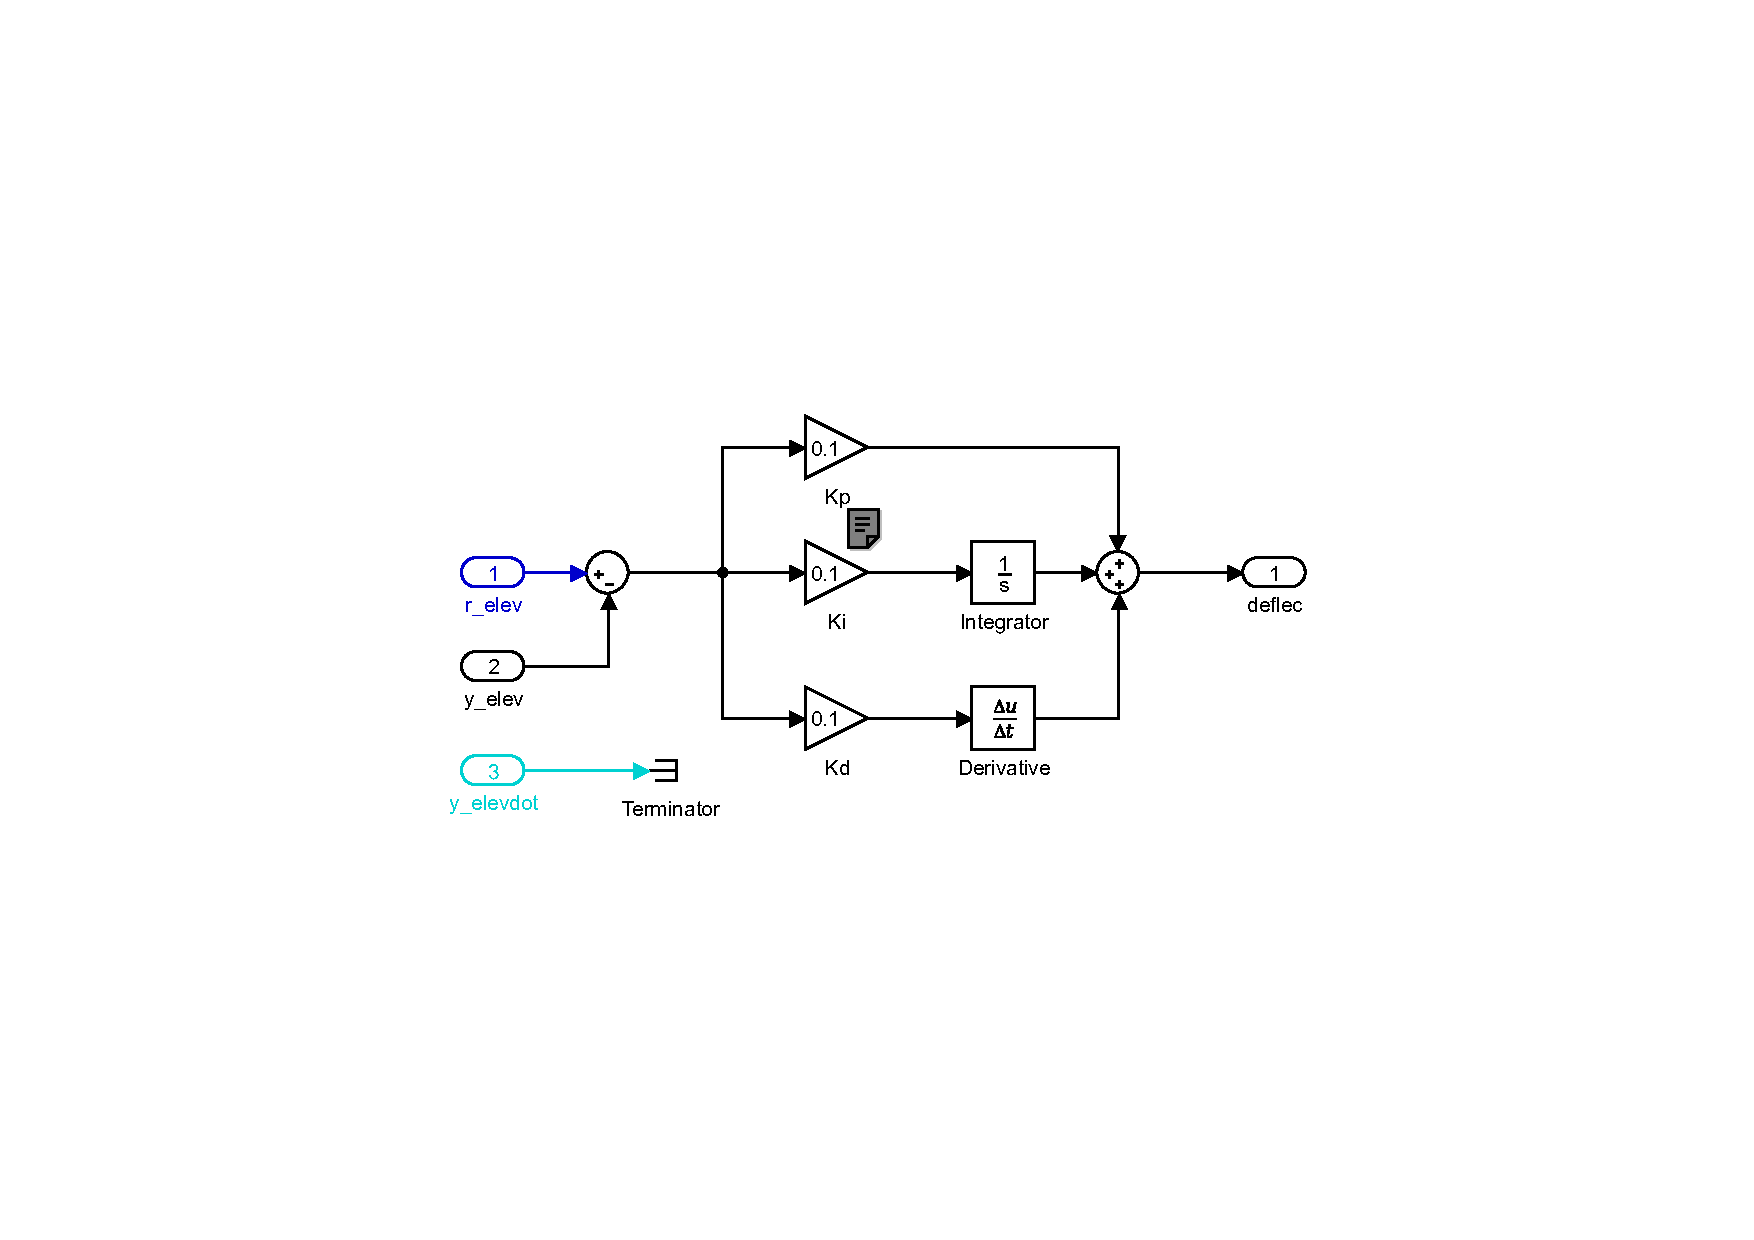
\includegraphics[trim = 0 0 0 0, clip, width=0.395\textwidth]{origcontrol.pdf}
\vspace{-10pt}
  \caption{Showing original Controller Architecture}
  \vspace{-25pt}
  \label{origcontrol}
 \end{wrapfigure}

In Quanser Control Part 3, the improved PID controller successfully met
the Phase 2 requirements but failed to meet the overshoot (OS) condition
for the desired controller. The PID control architecture in Figure
\ref{origcontrol} from Part 2 was tested using both non-linear
simulation and on the Quanser setup.

\begin{wrapfigure}{r}{0.4\textwidth}
 \vspace{-25pt}
 \centering
  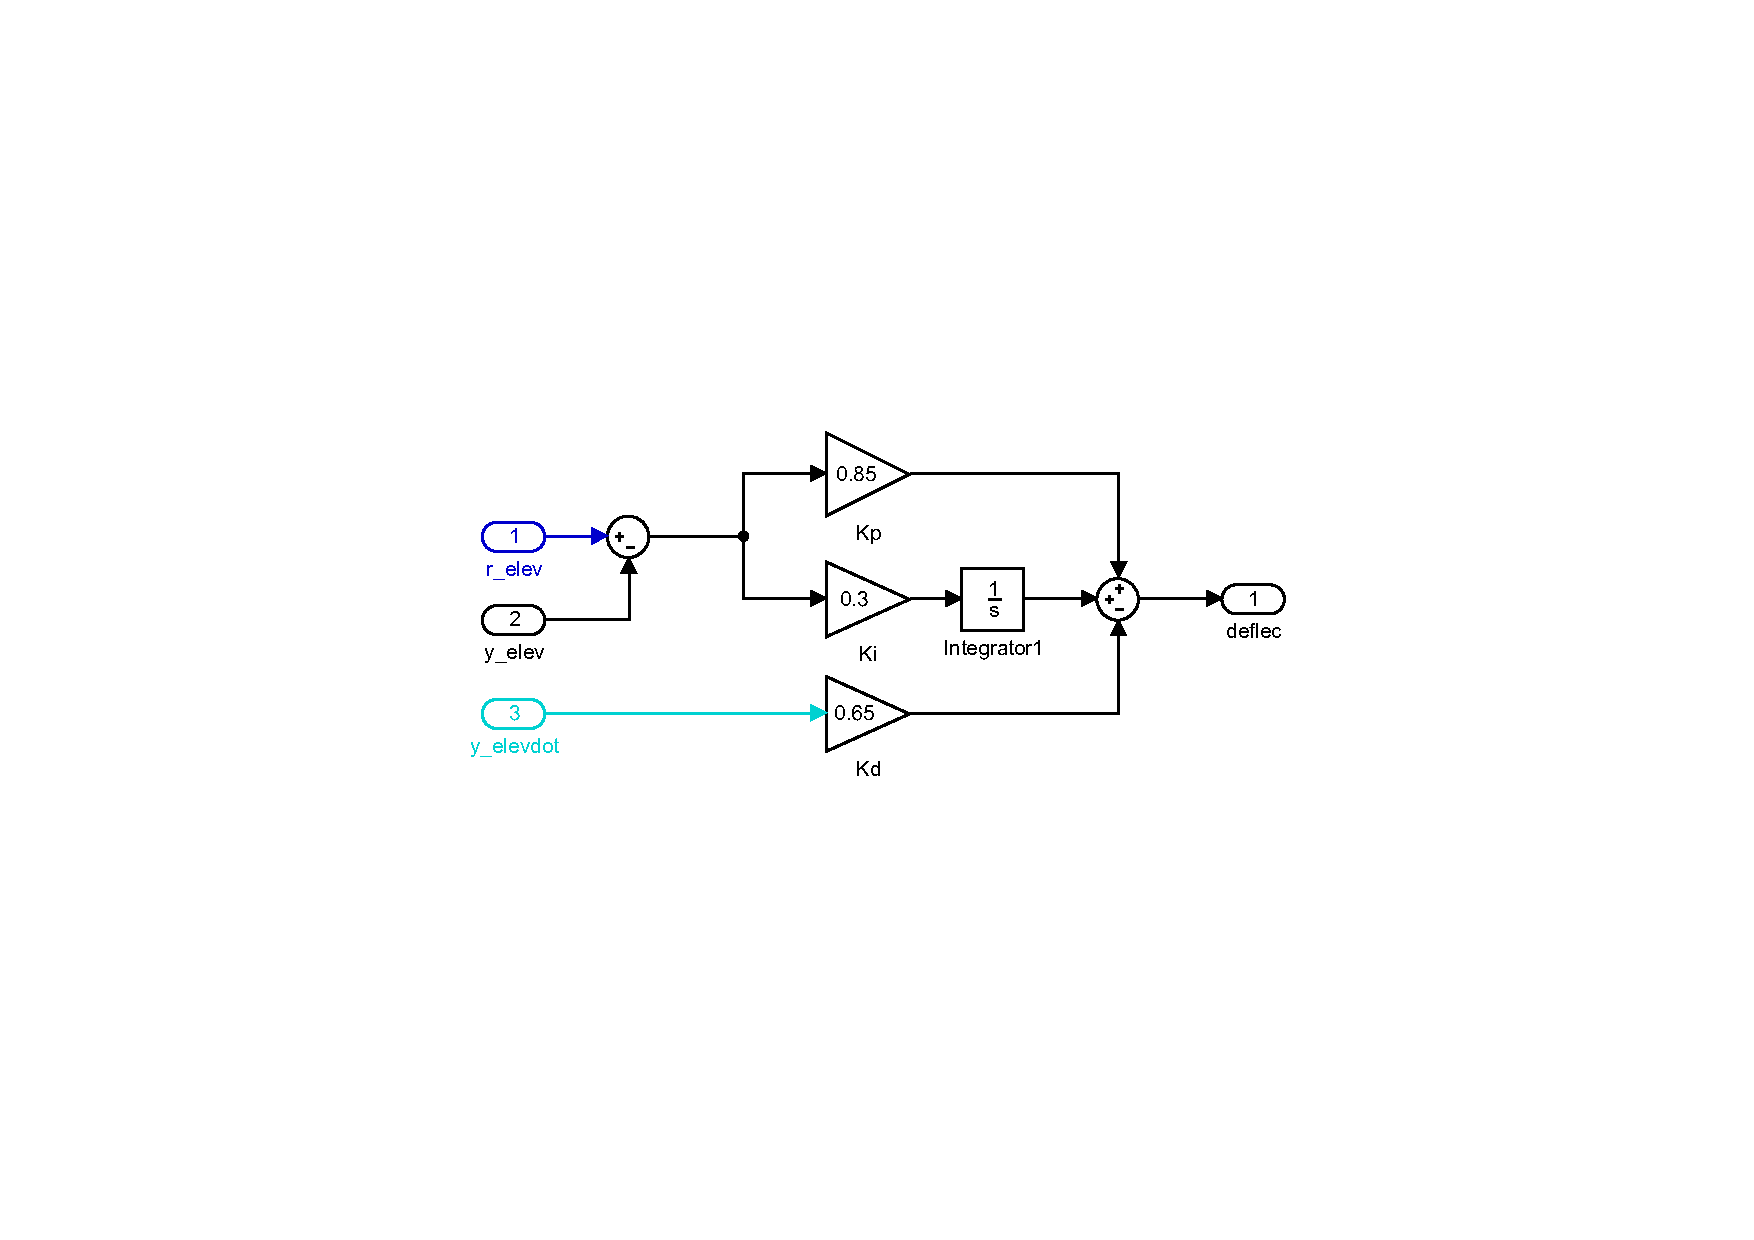
\includegraphics[trim = 0 0 0 0, clip, width=0.395\textwidth]{fincontrol.pdf}
\vspace{-10pt}
  \caption{Showing Improved Controller Architecture}
  \vspace{-20pt}
  \label{fincontrol}
 \end{wrapfigure}

At this stage, the design process for the controller consisted of;
extracting preliminary responses from the Quanser-rig, analysing the
responses to obtain a simulated plant transfer function. The transfer
function was designed to represent small changes in elevation angle,
whereby selection of the controller architecture and gains, manifested a
desirable response. The controller, therefore, was built to achieve a
good response in the simulation, but is susceptible to errors when
translating to the real Quanser-rig based the limitations in the
assumption made.

To meet the overshoot requirement, the controller was further refined in
the original simulation. Using understanding taken from Phase 2, shown
in Table \ref{paramtab}, gains were modified to improve the results
further. The integrator gain (\(K_i\)) has the greatest effect on the
steady-state error. \(K_i\) was first increased by an increment, until
the transfer function response began to deteriorate. \(K_i\) had only a
small range in which the response could be altered without degrading the
results; suggesting that the original \(K_i\) value was a good fit.
Maximising \(K_i\) first, meant that the effects of varying derivative
gain (\(K_d\)) on the steady state would be minimised. A similar process
was followed for then the proportional gain (\(K_p\)) and \(K_d\), where
\(K_p\) was maximised to reduce the rise time (\(T_R\)) and \(K_d\) was
optimised to reduce the overshoot. Maximising these values, helped
improve the performance characteristics without heavily deteriorating
other properties.

\begin{wrapfigure}{r}{0.42\textwidth}
 \vspace{-35pt}
\centering
\captionof{table}{Effect of Increasing PID Gains on Objectives}
\vspace{-2pt}
 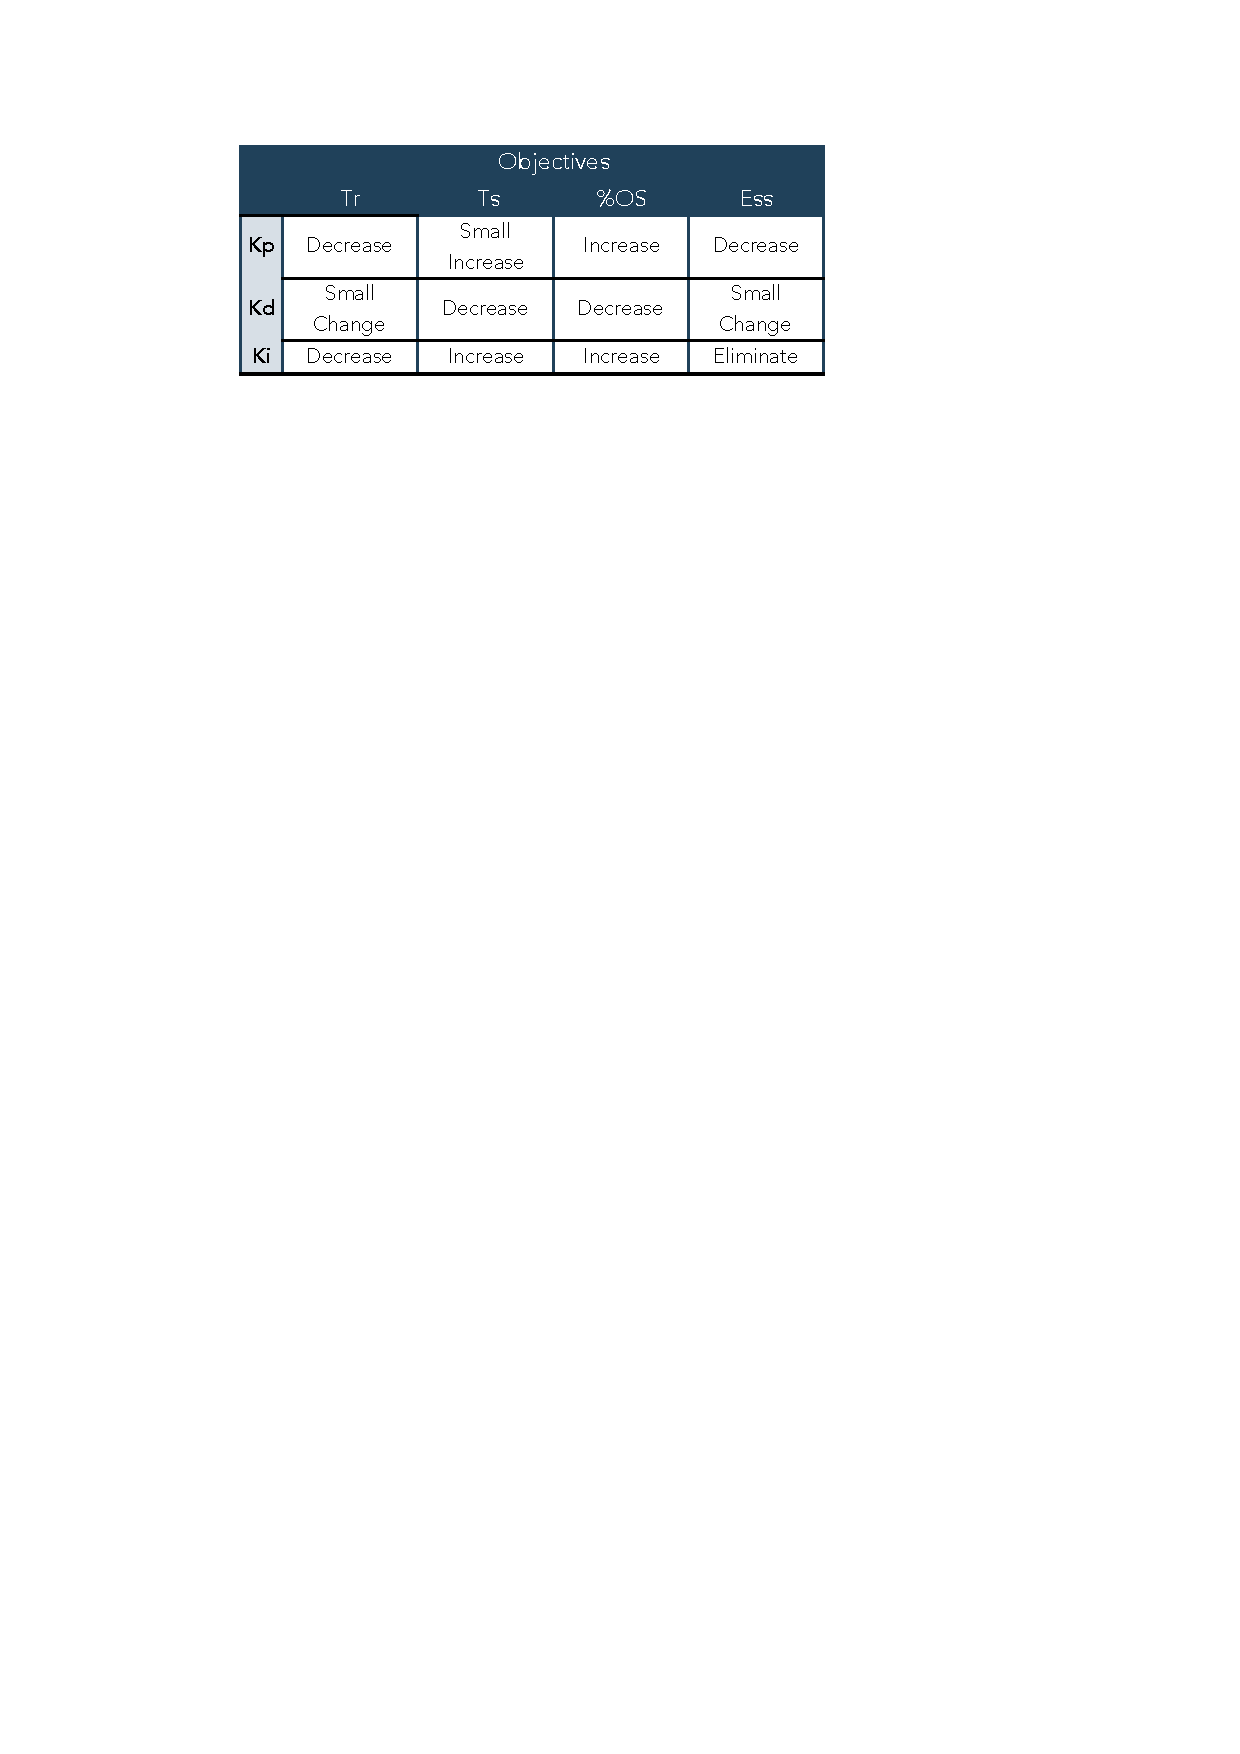
\includegraphics[trim = 0 0 0 0, clip, width=0.419\textwidth]{tableobj.pdf}
 \vspace{-35pt}
 \label{paramtab}
 \end{wrapfigure}

To test the controller performance more vigorously, the PID was run in a
new simulation, with non-linearities added; in the form of a rate
limiter and saturation block. A rate limiter limits the speed of change
of the signal, while the saturation block represents a limit in
amplitude. This new simulation would improve the accuracy of the
expected Quanser response emulation. A marginal change could be seen
when comparing the results of the non-linear simulation to the original,
where overshoot would increase slightly. Further experimentation found
that increasing gain values by an order of magnitude, destabilised the
results revealing much greater non-linear effects. This observation
confirmed that the PID gains selected fell within an acceptable region.
With a small additional tweaking following the same design process, the
final gain values shown in Table \ref{gains} met the requirements of the
Phase 3 design characteristics.

\begin{wrapfigure}{r}{0.255\textwidth}
\vspace{-30pt}
 \centering
  \captionof{table}{Showing Controller Gain Values Used}
 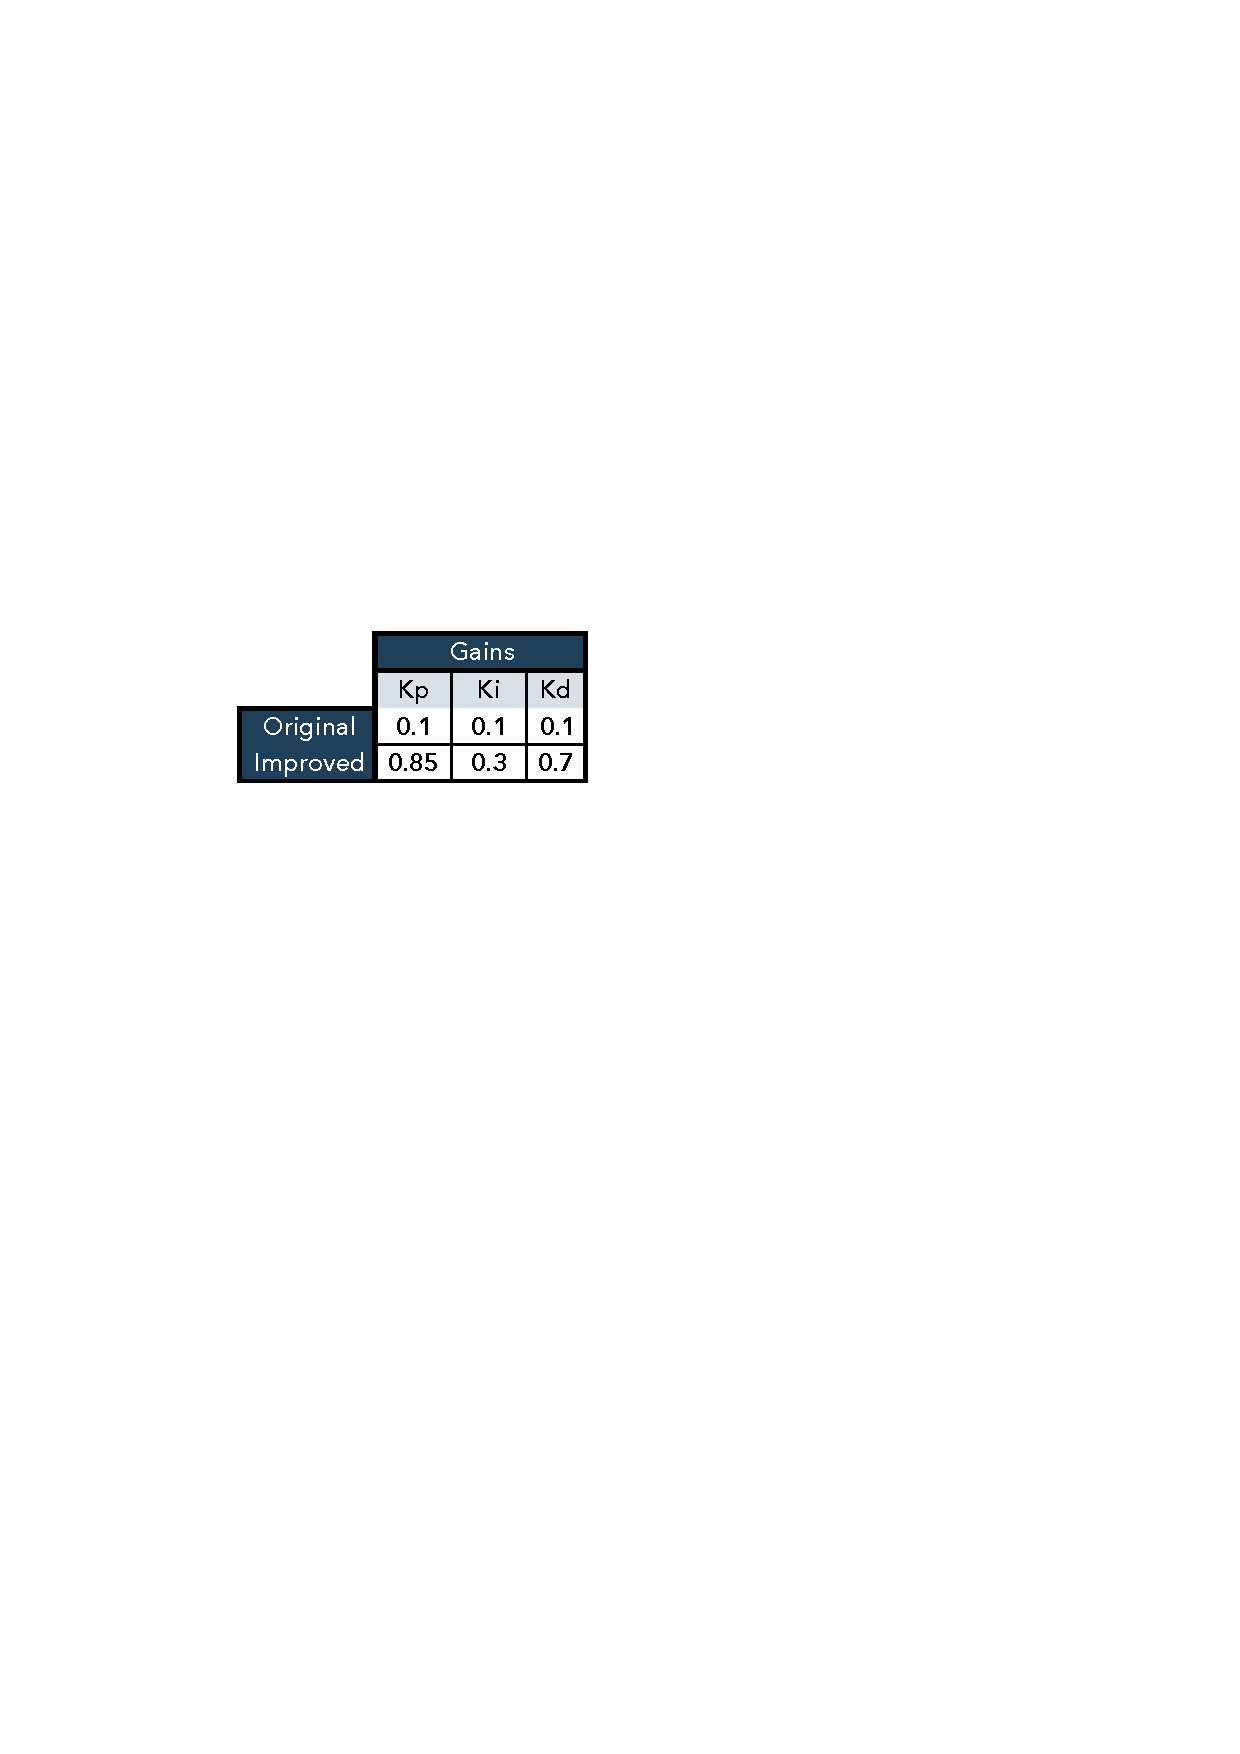
\includegraphics[trim = 0 0 0 0, clip, width=0.254\textwidth]{gains2.pdf}
 \label{gains}
\vspace{-20pt}
 \end{wrapfigure}

Figure \ref{fincontrol} shows the original controller configuration
utilised the numerical Simulink derivative block within the PID
controller. It was found that the control architecture could also be
improved for the actual control rig. Using the derivative as output
directly \texttt{y\_elevdot} from the Quanser - it was expected that the
numerical derivative block would not be as representative of the
observed rate of change as the actual derivative output. This view was
confirmed by the improved experimental results from provisional testing
on the Quanser-Rig. The difference in architecture was unobservable in
simulation, highlighting a noticeable difference between real and
simulated output data.

\section{Quanser Controller
Refinements}\label{quanser-controller-refinements}

After satisfying the desired requirements in the non-linear simulation,
the controller tests were conducted on the Quanser-rig. The controller
performed well, meeting the desired requirements, where a small
improvement in overshoot could be observed from the simulation. Due
sampling errors, small deviations from the steady state could be seen
(see \ref{quanscomp}) of \(\pm 0.4\)\% could be seen from elevation
angle. As the sampling rate was limited by the sensors on the Quanser,
results appeared jagged. This reducing the precision of the results but
was small enough, for the results to represent the response of the
Quanser to enough accuracy.

\section{Results}\label{results}

\begin{figure}[H]
 \centering
 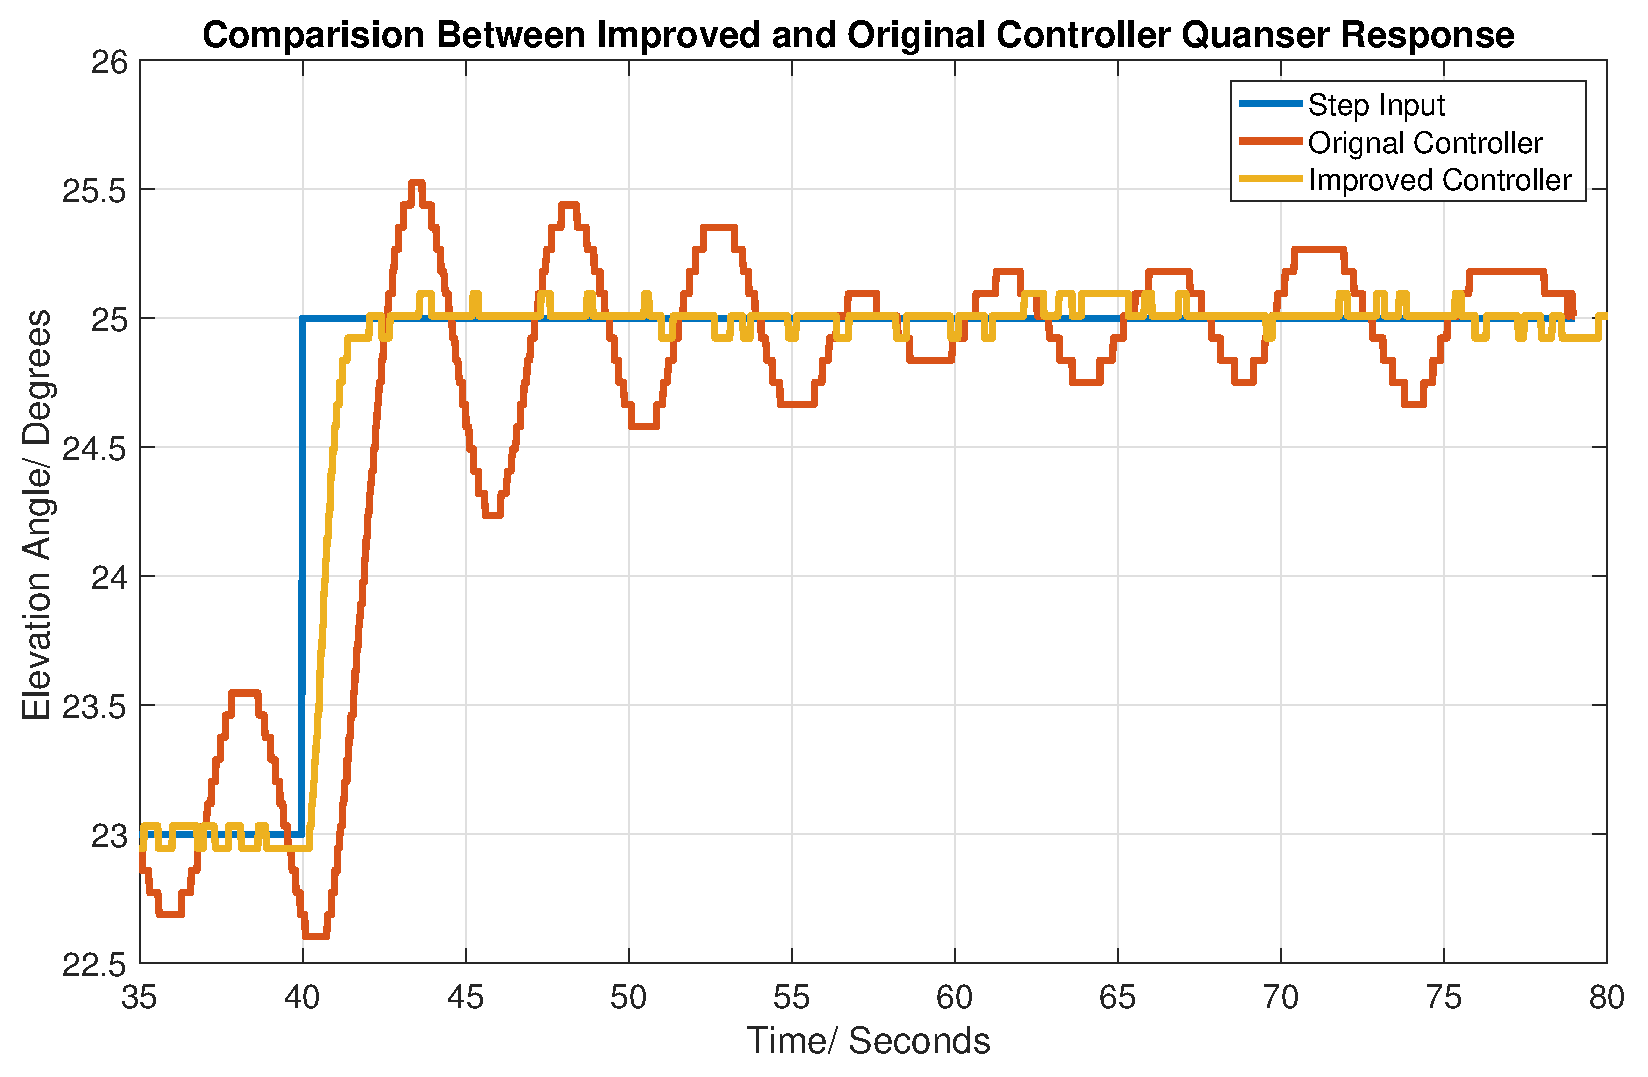
\includegraphics[trim = 0 0 0 0, clip, width=0.8\textwidth]{quanscomp.eps}
\caption{Showing Difference in Original and Improved Controller Performance on Quanser Response}
 \label{quanscomp}
 \end{figure}

\begin{figure}[H]
\centering
\begin{minipage}{.49\textwidth}
\centering
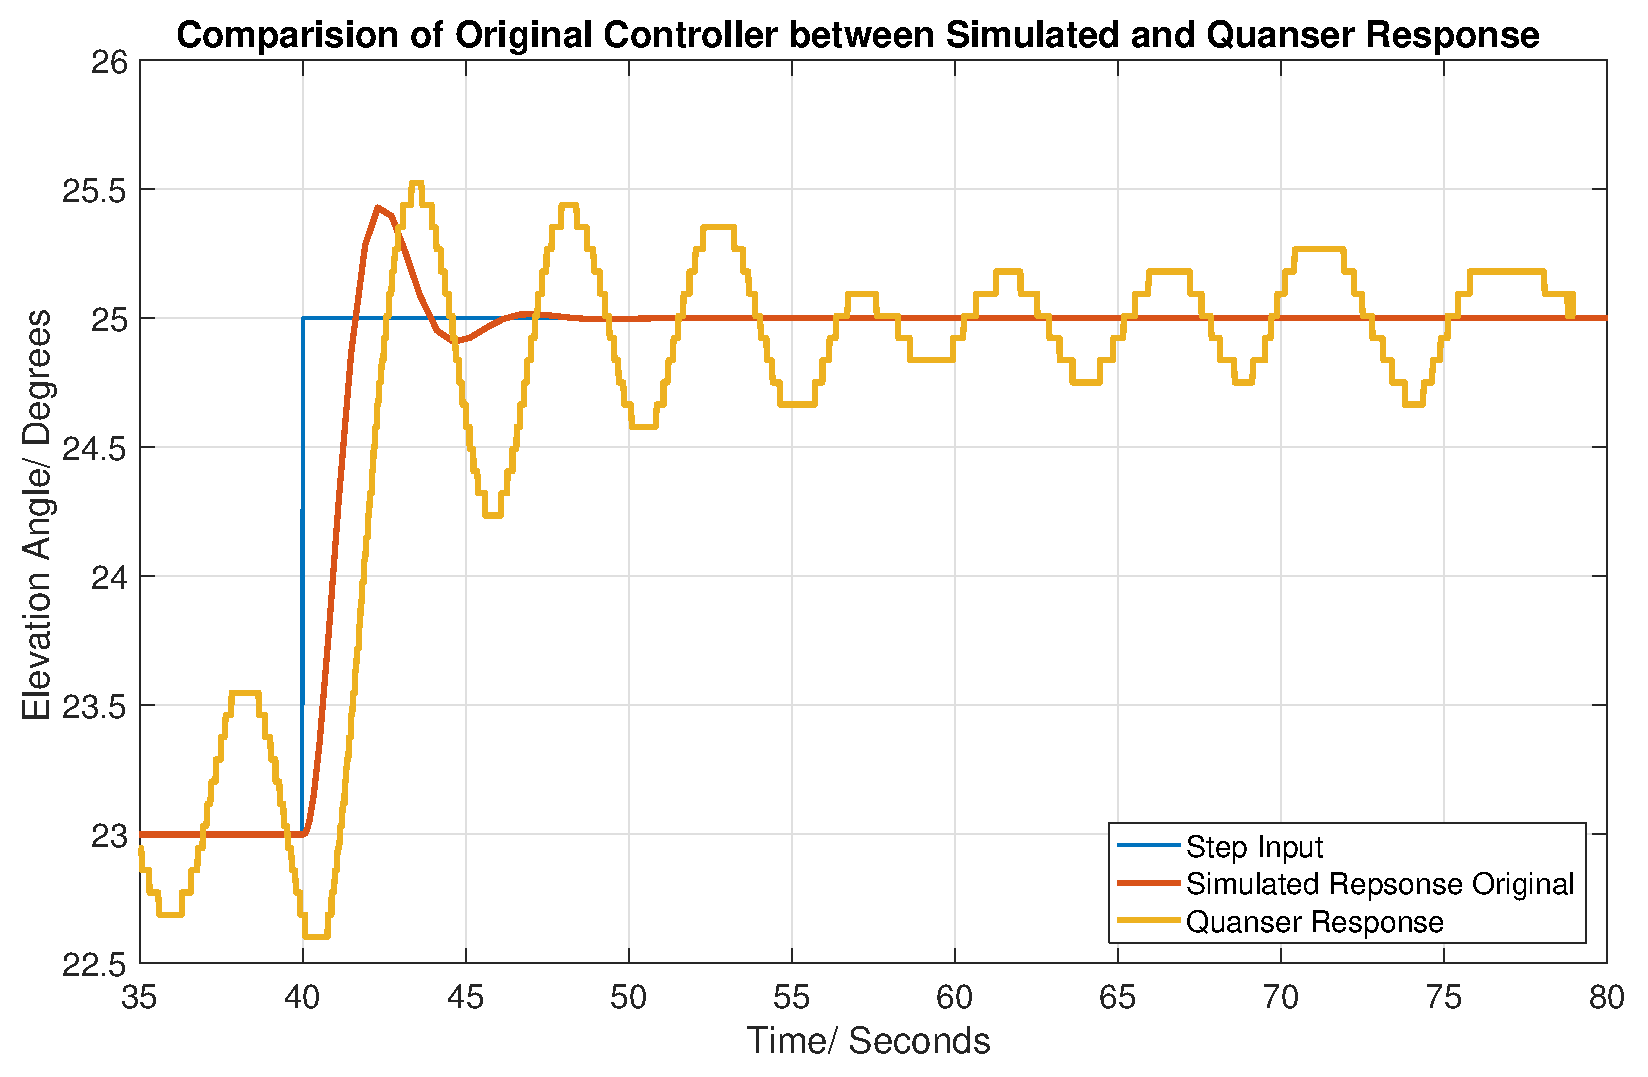
\includegraphics[trim = 0 0 0 0, clip, width=1\textwidth]{origresult.eps}
\caption{Showing Difference in Original Controller Performance Comparing Simulated and Quanser Responses}
\label{origresult}
\end{minipage}
\hfill
\begin{minipage}{.49\textwidth}
\centering
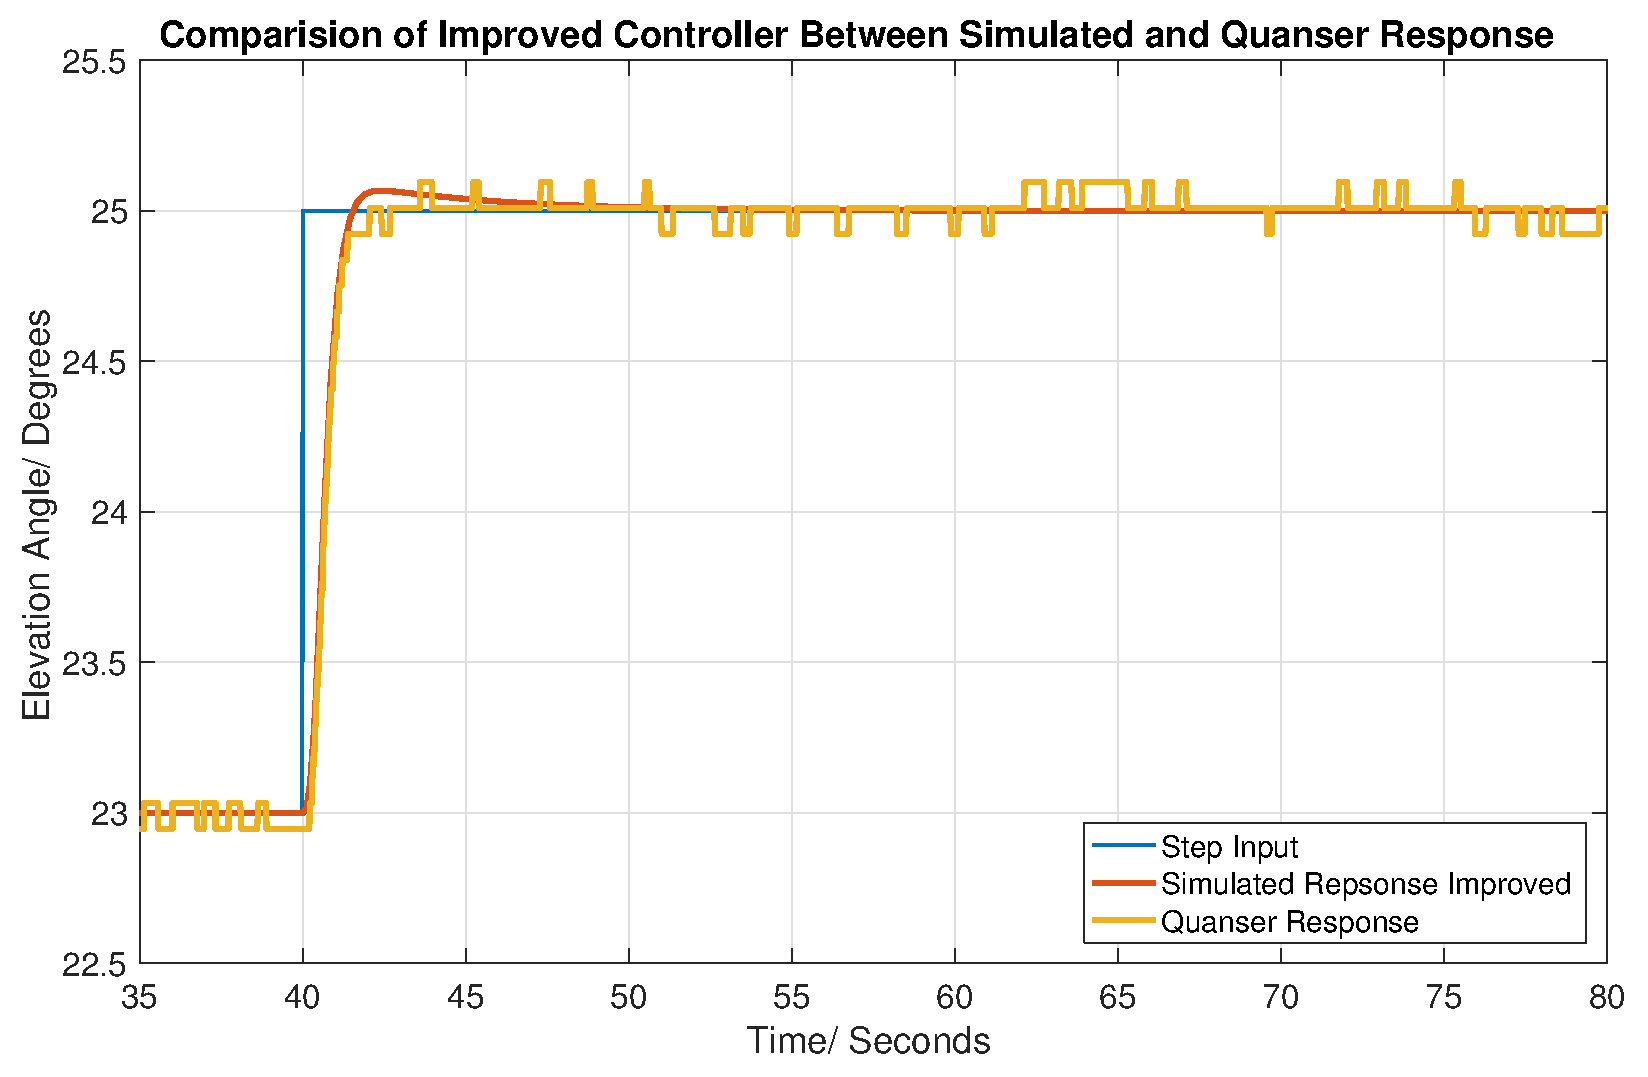
\includegraphics[trim = 0 0 0 0, clip, width=1\textwidth]{improvresult.eps}
\caption{Showing Difference in Improved Controller Performance Comparing Simulated and Quanser Responses}
\label{improvresult}
\end{minipage}
\vspace{-20pt}
\end{figure}

\begin{table}[H]
 \centering
 \caption{Showing Controller Response Results for Simulation and Quanser Tests}
 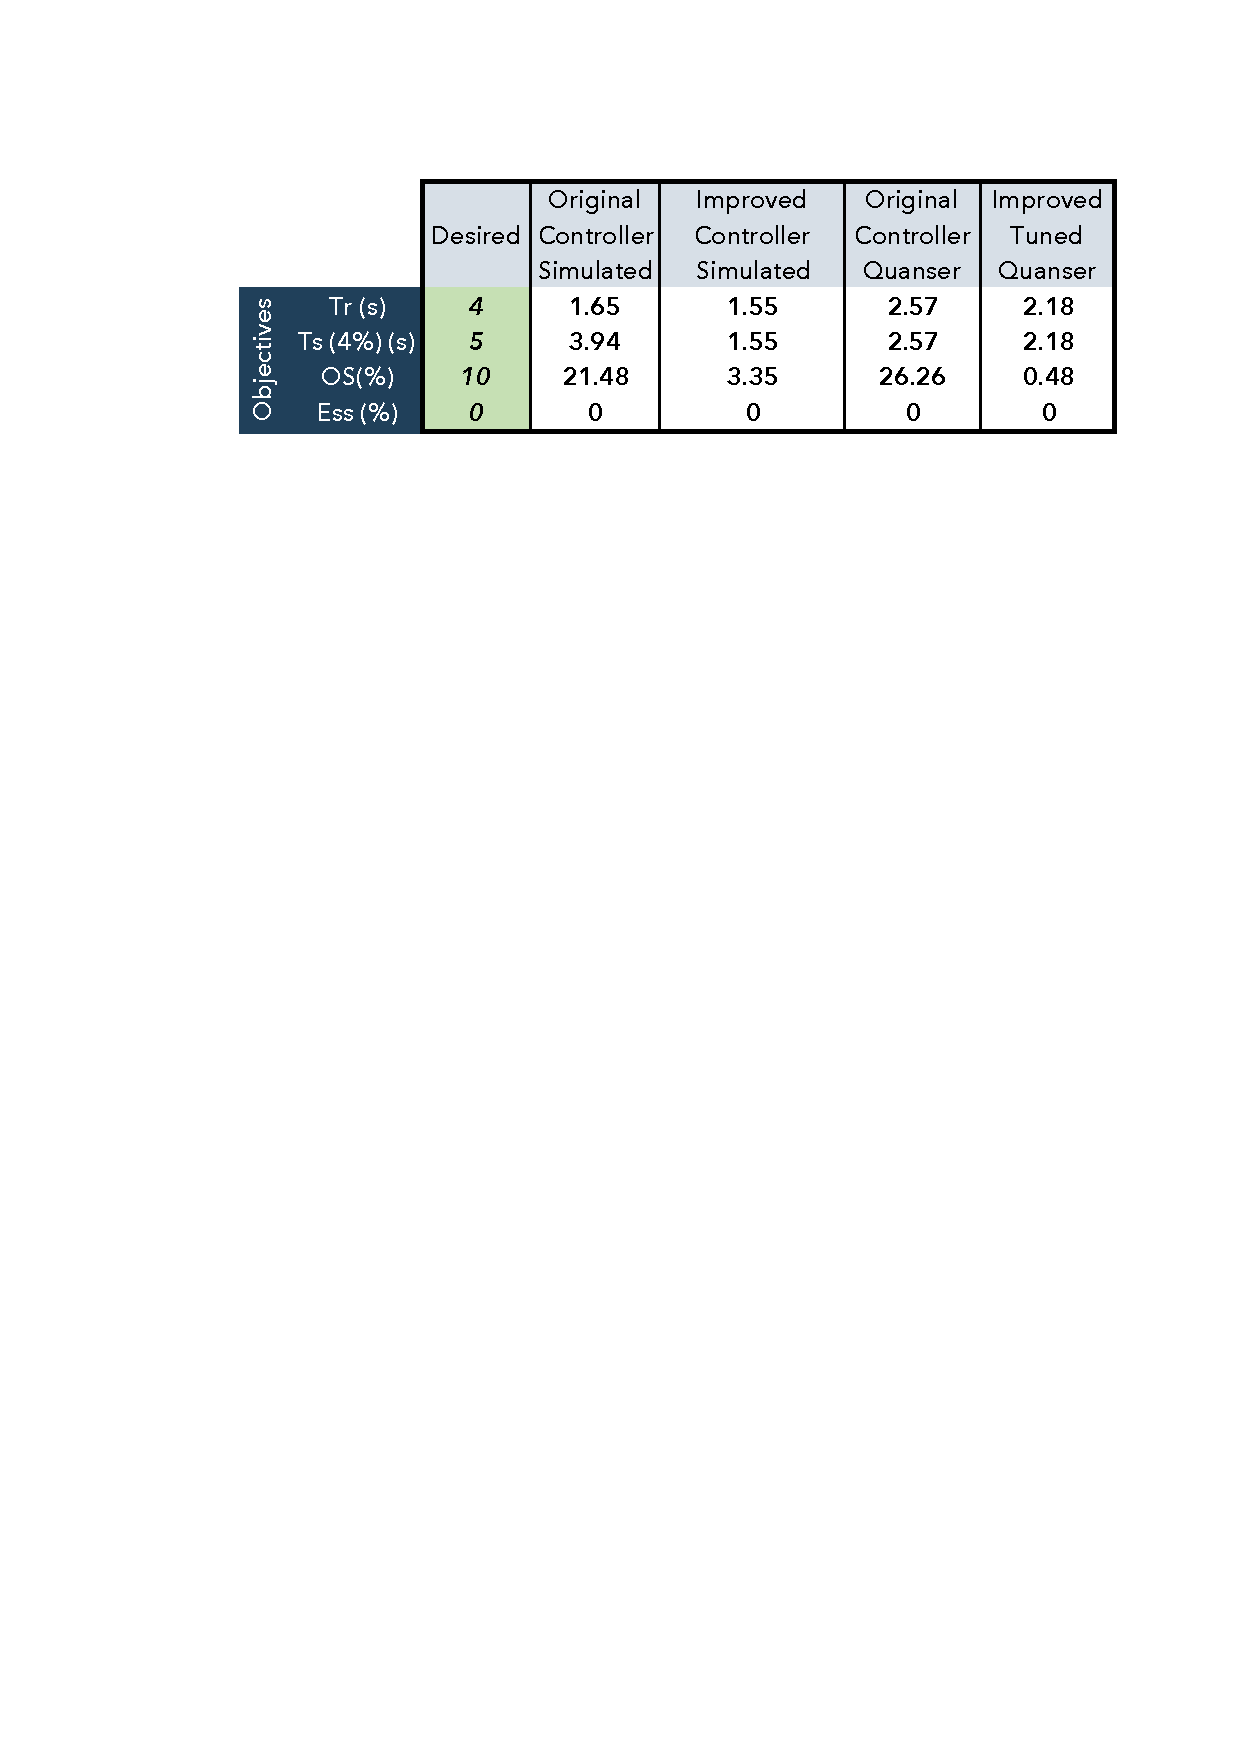
\includegraphics[trim = 0 0 0 0, clip, width=0.65\textwidth]{resultstab2.pdf}
 \label{resultstab}
 \end{table}

\section{Discussion}\label{discussion}

Figure \ref{quanscomp} highlights the experimental difference between
the original tuned PID controller (taken directly from Part 2) and the
iteratively improved (with an alternative architecture) PID controller.
The improved controller displayed a rise time of 2.18 seconds, settling
time of 2.18 seconds (as the 4\% error limits were satisfied at the same
time as the rise time), an Overshoot of 0.48\% and a negligible steady
state error. The natural Quanser response to a step input (from Part 1)
showed a sinusoidal response with large decaying amplitudes at high
frequencies. The designed controller improved on this undesirable
behaviour by increasing damping, and improving control of low amplitude
oscillations. These values comfortably satisfied the required
objectives, improving upon the desired objectives shown in Table
\ref{resultstab}. The improved controller showed a faster rise time,
settling time and reduced overshoot percentage over the original
controller design. In an engineering context, it is critical that the
controller response is sharp and responsive, minimising delay times.
Observing the step input time in Figure \ref{quanscomp}, it is evident
that the choice of the controller effects the delay and error of the
Step response.

The Quanser was allowed to settle after take-off to a reasonable level
before the step input was tested. Using the same settling time-period,
the original controller showed larger settling oscillations, this likely
contributed towards the amplitude and phase error displayed in
\ref{origresult} between the simulated Quanser response and the
experimental Quanser response. This observation is also reinforced by
Figure \ref{improvresult} as the Simulink step input shows less delay.
If the step was placed mid oscillations, this difference from the
steady-state would add to the step response. This effect is likely to be
present in real world rotatory wing aircraft. Design parameters were
estimated conservatively to meet the requirements in any case.

Idealisation of the elevator actuation could also be observed when
comparing the simulation to real world response. It was assumed that no
physical limitations are in place on the system. Realistically, this may
be misrepresenting the physical actuator, likely introducing errors in
the form of actuator delay.

The results presented above highlight the step response for the tuned
PID controller for a step input of 2, chosen as the transfer function
was derived from experimental results of elevator angle step changes
between -2 and 2. It is expected that for step inputs out of this range,
the tuned controller will perform sub-optimally; accurate near the
`fix-point' and showing deviations at higher step inputs.

Figure \ref{ampres} shows the magnitude of rate of response for the
Quanser-rig. It can be observed that the action (in terms of magnitude)
and speed (showing thick solid band) are both adequate for the
controller. This observation further confirms the correct magnitude of
gains were selected for the controller as rate and magnitude are both
within the limits of the Quanser performance.

\begin{wrapfigure}{r}{0.45\textwidth}
\vspace{-10pt}
\centering
 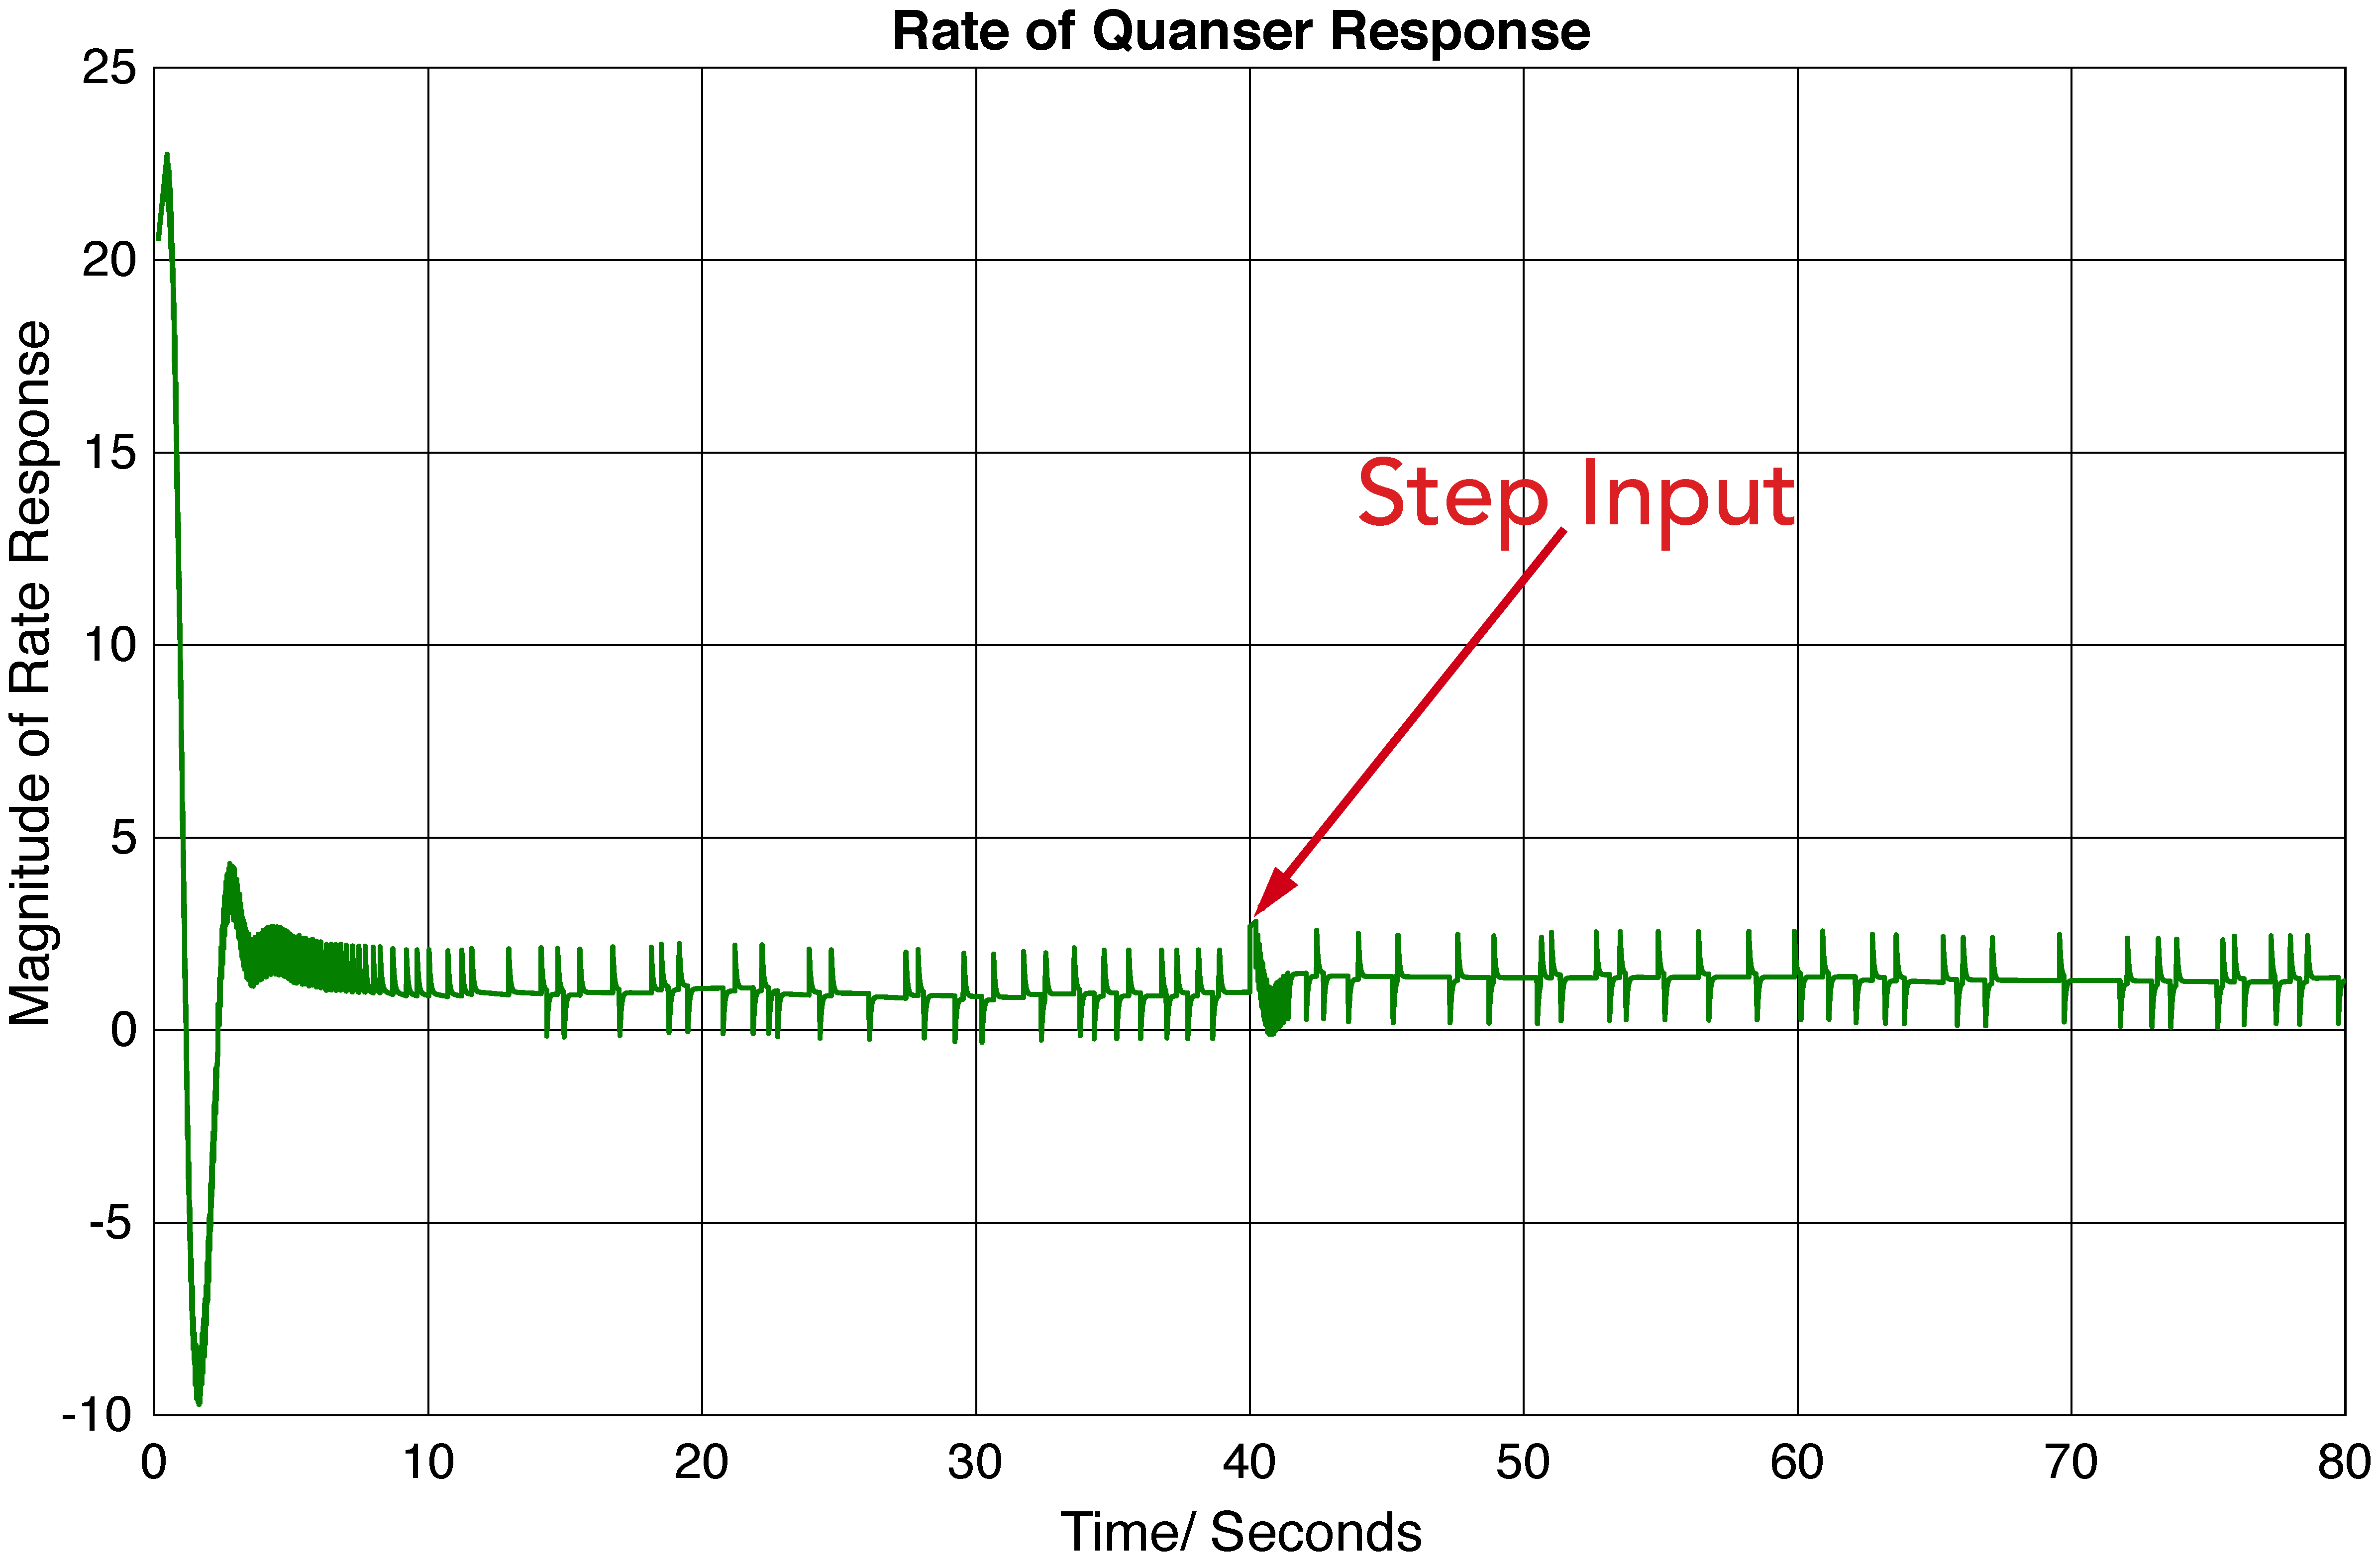
\includegraphics[trim = 0 0 0 0, clip, width=0.45\textwidth]{ampresmark2.eps}
\vspace{-5pt}
\caption{Showing Magnitude of Rate Response}
 \vspace{-20pt}
 \label{ampres}
\end{wrapfigure}

The Quanser-rig tests were set in a reasonably controlled environment
with few assumed non-linearities from these setup conditions. The PID,
therefore, was designed assuming that all non-linearities were weak. The
controlled environment meant the tuning process was simple allowing the
specified requirements to be met. In more complex engineering
applications, the system in question may display a larger number of
non-linear effects. This may be accounted for using the method of gain
scheduling. Gain Scheduling \cite{stackcont} achieves control of a
non-linear system by linearising the problem at various operation
states; resulting in a ``family'' of PID controllers which will each
respectively activate when a certain operation state is achieved. Each
of these PID controllers must be tuned independently to optimise for
their respective linearisation. The design then switches between each of
these models to achieve the ``best response'' for the current state.
More conclusively, within limits of this study, the obtained tuned PID
controller for the Quanser is effective and meets the desired time
domain requirements. For further accuracy of either Quanser control or
more complex systems; additional control structures should be
considered, particularly if the controller should encompass less stable
operations such as take-off and landing. In an aircraft control context,
the control parameters may be altitude or Mach.

\section{Conclusions}\label{conclusions}

This experiment has been a useful exercise in illustrating methods and
common pitfalls when transferring a theoretically functioning PID
controller to a real world system. Predicting the Quanser response using
a non-linear simulation, allows for a good controller to be created but
exact characteristics are difficult to predict without real-world
experimentation. Further controller refinement is therefore required
when transferring to the real system, using the simulation as a method
of getting close to the answer. It was interesting to note that the real
world response always varied from the expected simulations for every
tested tuned PID controller and configuration - this difference is
likely to be an artefact of the non-linearities present in the
Quanser-rig.
